\documentclass[tikz]{standalone}
\usetikzlibrary{arrows, positioning}
\usetikzlibrary{calc,shapes.multipart,chains}
\usetikzlibrary {arrows.meta}
\usepackage{xcolor}
\definecolor{allcolor}{RGB}{148,182,233}
\newcommand*{\equal}{=}
\tikzset{
  treenode/.style = {align=center, inner sep=1pt, text centered,
    font=\sffamily},
  bst/.style = {treenode, circle, black, font=\sffamily\bfseries, draw=black, text width=2em}
}
\begin{document}
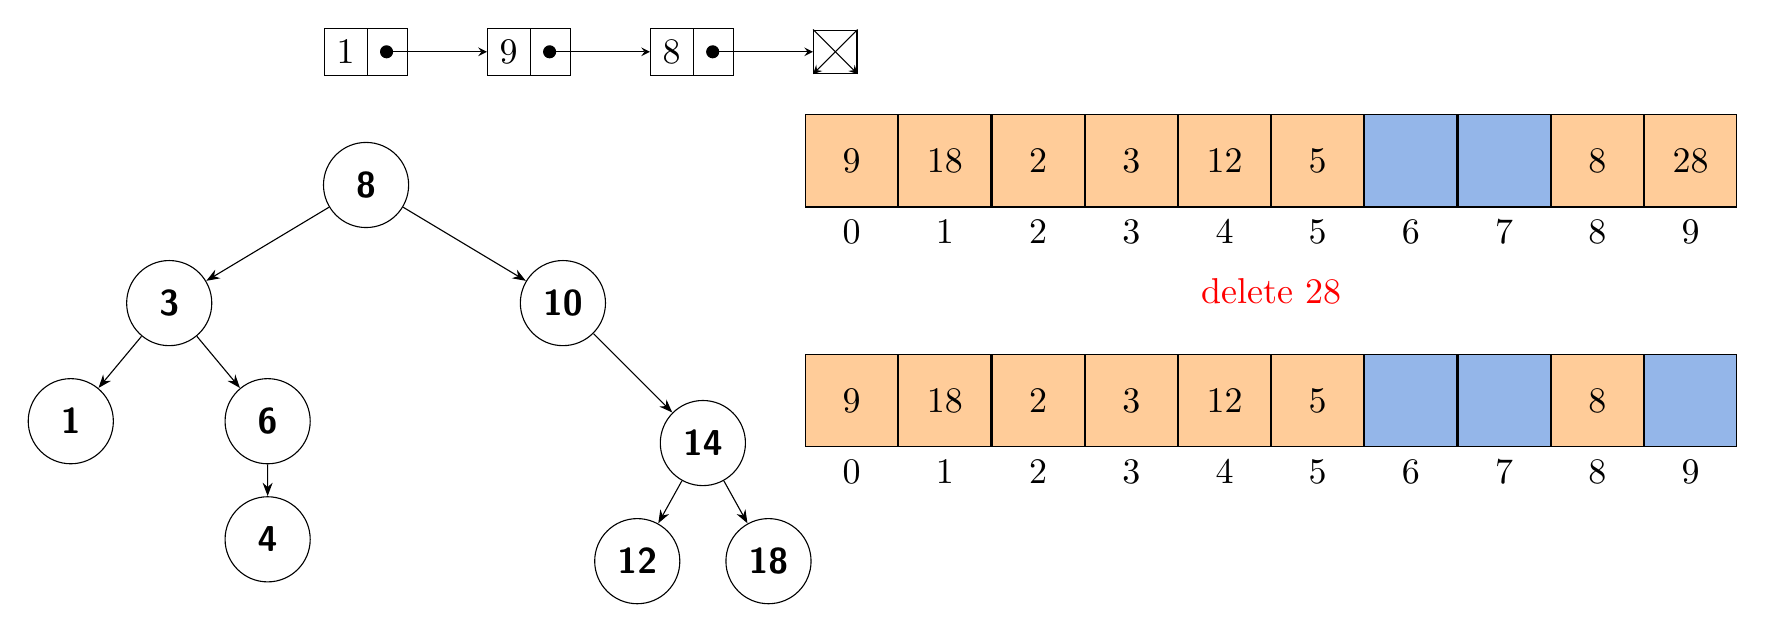
\begin{tikzpicture}[->,>=stealth',level/.style={sibling distance = 5cm/#1,
  level distance = 1.5cm}, every node/.style={scale=1.3}, dot/.style={minimum size=0.1mm, circle, fill=black!90}, slot/.style={minimum size=0.9cm, rectangle}, noslot/.style={slot, fill=allcolor},
  yesslot/.style={slot, fill=orange!40}, data/.style={minimum size=0.7cm, fill=orange!40}, >=Stealth]
\node (n8) [bst] {8}
    child {node [bst] {3}
        child {node [bst] {1}}
        child {node [bst] {6}
            child {node [bst] {4}}
        }
    }
    child {node (n10) [bst] {10}
        child {node [bst, below right=of n10] {14}
            child {node [bst] {12}}
            child {node [bst] {18}}
        }
    }
;
\tikzstyle{textbf} = [text width=5cm,text centered]

\matrix [row sep=1cm,nodes=draw, right=of n8, xshift=3cm] (table1)
{
  \node[yesslot, label=below:$0$] {9}; &
  \node[yesslot, label=below:$1$] {18}; &
  \node[yesslot, label=below:$2$] {2}; &
  \node[yesslot, label=below:$3$] {3}; &
  \node[yesslot, label=below:$4$] {12}; &
  \node[yesslot, label=below:$5$] {5}; &
  \node[noslot, label=below:$6$] {}; &
  \node[noslot, label=below:$7$] {}; &
  \node[yesslot, label=below:$8$] {8}; &
  \node[yesslot, label=below:$9$] {28}; &
  \\
}; 

\matrix [row sep=1cm,nodes=draw, below=of table1] (table0)
{
  \node[yesslot, label=below:$0$] {9}; &
  \node[yesslot, label=below:$1$] {18}; &
  \node[yesslot, label=below:$2$] {2}; &
  \node[yesslot, label=below:$3$] {3}; &
  \node[yesslot, label=below:$4$] {12}; &
  \node[yesslot, label=below:$5$] {5}; &
  \node[noslot, label=below:$6$] {}; &
  \node[noslot, label=below:$7$] {}; &
  \node[yesslot, label=below:$8$] {8}; &
  \node[noslot, label=below:$9$] {}; &
  \\
}; 

\node [above=of table0, red, yshift=-0.5cm] {delete $28$};

\begin{scope}[below=of table1, yshift=2cm, list/.style={rectangle split, rectangle split parts=2,
    draw, rectangle split horizontal}, >=stealth, start chain]
\node[list,on chain] (A) {1};
\node[list,on chain] (B) {9};
\node[list,on chain] (C) {8};
\node[on chain,draw,inner sep=6pt] (D) {};
\draw (D.north east) -- (D.south west);
\draw (D.north west) -- (D.south east);
\draw[*->] let \p1 = (A.two), \p2 = (A.center) in (\x1,\y2) -- (B);
\draw[*->] let \p1 = (B.two), \p2 = (B.center) in (\x1,\y2) -- (C);
\draw[*->] let \p1 = (C.two), \p2 = (C.center) in (\x1,\y2) -- (D);
\end{scope}
\end{tikzpicture}
\end{document}
